% !TEX root = FDS_Validation_Guide.tex

\chapter{Wind Engineering and Atmospheric Dispersion}

This chapter presents results of simulations of wind over structures and atmospheric dispersion, all involving a simplified atmospheric boundary layer model in FDS.


\section{UWO Wind Tunnel Experiments}

A description of the UWO Wind Tunnel experiments is included in Sec.~\ref{UWO_Wind_Tunnel_Description}. Schematic drawings of the wind tunnel models are shown in Fig.~\ref{UWO_Drawings}.

Figures~\ref{UWO_Test_7_pressure_coefficients_180_1} through \ref{UWO_Test_7_pressure_coefficients_270_2} show comparisons of measured and predicted mean, rms, minimum and maximum values of the pressure coefficients on the surface of a 1:100 scale model of a building in a wind tunnel. The model building is shown at the top of Fig.~\ref{UWO_Drawings}. Figures~\ref{UWO_SS21_Test_6_pressure_coefficients_0_1} through \ref{UWO_SS21_Test_6_pressure_coefficients_45_4} show similar results for the model shown at the bottom of Fig.~\ref{UWO_Drawings}. The comparisons are made for two wind directions for each model. For SS20-Test~7, the 180$^\circ$ wind direction is perpendicular to the model's shorter side. The 270$^\circ$ wind direction is perpendicular to the model's longer side. For the SS21-Test~6 model, the wind directions are 0$^\circ$ (perpendicular to short side) and 45$^\circ$.

The diagrams in Fig.~\ref{UWO_Drawings} indicate the location of the ``lines'' where the data is compared. The discontinuities in the lines represent the transition from the windward side, to the roof, to the leeward side. The side plots do not include windward or leeward side data.

The simulations are run for approximately one-tenth the time as that of the experiments, which were run for 100~s. The minimum and maximum values for the simulations are extrapolated so that they may be compared to the measured min and max for the 100~s experiment. The procedure is described in the FDS User's Guide~\cite{FDS_Users_Guide}, in the section describing the {\ct TEMPORAL\_STATISTIC} {\ct 'MIN'} and {\ct 'MAX'}.

\begin{figure}[!ht]
\centering
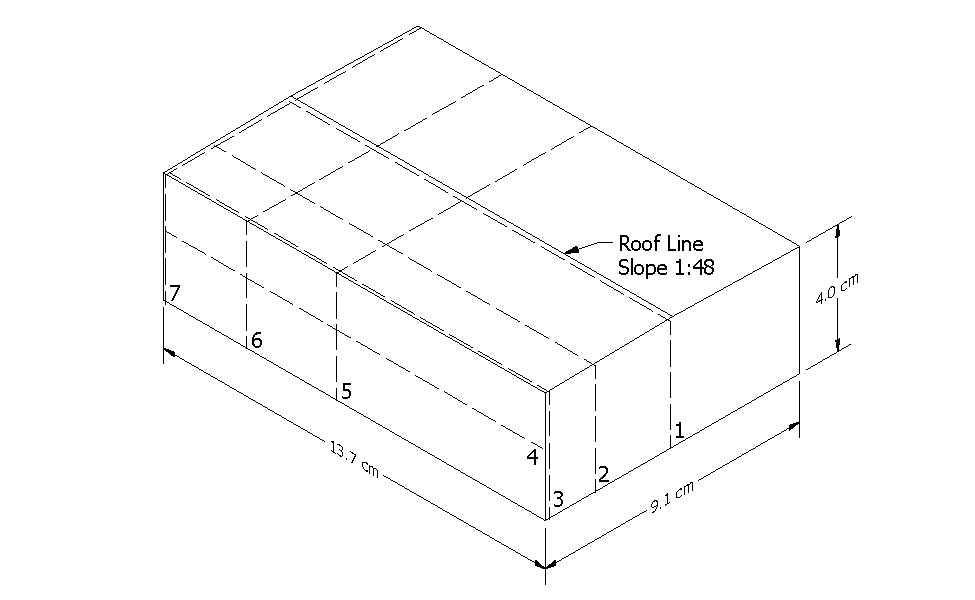
\includegraphics[width=5.5in]{FIGURES/UWO_Wind_Tunnel/UWO-BLT-SS20-Test7}
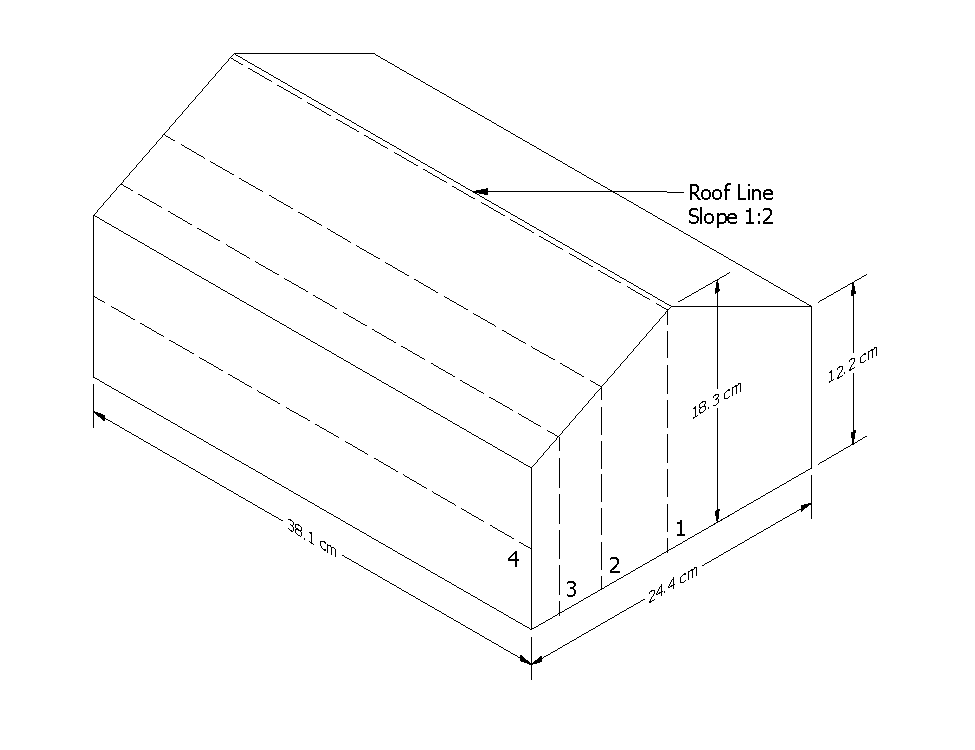
\includegraphics[width=5.5in]{FIGURES/UWO_Wind_Tunnel/UWO-BLWT-SS21-Test6-40ft}
\caption[UWO Wind Tunnel schematic drawings]{UWO Wind Tunnel schematic drawings. (Top) SS20-Test 7. (Bottom) SS21-Test 6. The numbers at the base of the models denote the starting points of the lines over which the measurements and predictions are compared.}
\label{UWO_Drawings}
\end{figure}

\begin{figure}[p]
\begin{tabular*}{\textwidth}{l@{\extracolsep{\fill}}r}
\includegraphics[height=2.1in]{SCRIPT_FIGURES/UWO_Wind_Tunnel/UWO_Cp_mean_180_line_1} &
\includegraphics[height=2.1in]{SCRIPT_FIGURES/UWO_Wind_Tunnel/UWO_Cp_rms_180_line_1} \\
\includegraphics[height=2.1in]{SCRIPT_FIGURES/UWO_Wind_Tunnel/UWO_Cp_min_180_line_1} &
\includegraphics[height=2.1in]{SCRIPT_FIGURES/UWO_Wind_Tunnel/UWO_Cp_max_180_line_1} \\
\includegraphics[height=2.1in]{SCRIPT_FIGURES/UWO_Wind_Tunnel/UWO_Cp_mean_180_line_2} &
\includegraphics[height=2.1in]{SCRIPT_FIGURES/UWO_Wind_Tunnel/UWO_Cp_rms_180_line_2} \\
\includegraphics[height=2.1in]{SCRIPT_FIGURES/UWO_Wind_Tunnel/UWO_Cp_min_180_line_2} &
\includegraphics[height=2.1in]{SCRIPT_FIGURES/UWO_Wind_Tunnel/UWO_Cp_max_180_line_2}
\end{tabular*}
\caption[UWO Wind Tunnel, SS20-Test 7 pressure coefficients, 180\si{\degree}]{UWO Wind Tunnel, SS20-Test 7 pressure coefficients, 180\si{\degree} wind direction.}
\label{UWO_Test_7_pressure_coefficients_180_1}
\end{figure}

\begin{figure}[p]
\begin{tabular*}{\textwidth}{l@{\extracolsep{\fill}}r}
\includegraphics[height=2.1in]{SCRIPT_FIGURES/UWO_Wind_Tunnel/UWO_Cp_mean_180_line_3} &
\includegraphics[height=2.1in]{SCRIPT_FIGURES/UWO_Wind_Tunnel/UWO_Cp_rms_180_line_3} \\
\includegraphics[height=2.1in]{SCRIPT_FIGURES/UWO_Wind_Tunnel/UWO_Cp_min_180_line_3} &
\includegraphics[height=2.1in]{SCRIPT_FIGURES/UWO_Wind_Tunnel/UWO_Cp_max_180_line_3} \\
\includegraphics[height=2.1in]{SCRIPT_FIGURES/UWO_Wind_Tunnel/UWO_Cp_mean_180_line_4} &
\includegraphics[height=2.1in]{SCRIPT_FIGURES/UWO_Wind_Tunnel/UWO_Cp_rms_180_line_4}  \\
\includegraphics[height=2.1in]{SCRIPT_FIGURES/UWO_Wind_Tunnel/UWO_Cp_min_180_line_4} &
\includegraphics[height=2.1in]{SCRIPT_FIGURES/UWO_Wind_Tunnel/UWO_Cp_max_180_line_4}
\end{tabular*}
\caption[UWO Wind Tunnel, SS20-Test 7 pressure coefficients, 180\si{\degree}]{UWO Wind Tunnel, SS20-Test 7 pressure coefficients, 180\si{\degree} wind direction.}
\label{UWO_Test_7_pressure_coefficients_180_2}
\end{figure}

\begin{figure}[p]
\begin{tabular*}{\textwidth}{l@{\extracolsep{\fill}}r}
\includegraphics[height=2.1in]{SCRIPT_FIGURES/UWO_Wind_Tunnel/UWO_Cp_mean_270_line_5} &
\includegraphics[height=2.1in]{SCRIPT_FIGURES/UWO_Wind_Tunnel/UWO_Cp_rms_270_line_5} \\
\includegraphics[height=2.1in]{SCRIPT_FIGURES/UWO_Wind_Tunnel/UWO_Cp_min_270_line_5} &
\includegraphics[height=2.1in]{SCRIPT_FIGURES/UWO_Wind_Tunnel/UWO_Cp_max_270_line_5} \\
\includegraphics[height=2.1in]{SCRIPT_FIGURES/UWO_Wind_Tunnel/UWO_Cp_mean_270_line_6} &
\includegraphics[height=2.1in]{SCRIPT_FIGURES/UWO_Wind_Tunnel/UWO_Cp_rms_270_line_6} \\
\includegraphics[height=2.1in]{SCRIPT_FIGURES/UWO_Wind_Tunnel/UWO_Cp_min_270_line_6} &
\includegraphics[height=2.1in]{SCRIPT_FIGURES/UWO_Wind_Tunnel/UWO_Cp_max_270_line_6}
\end{tabular*}
\caption[UWO Wind Tunnel, SS20-Test 7 pressure coefficients, 270\si{\degree}]{UWO Wind Tunnel, SS20-Test 7 pressure coefficients, 270\si{\degree} wind direction.}
\label{UWO_Test_7_pressure_coefficients_270_1}
\end{figure}

\begin{figure}[p]
\begin{tabular*}{\textwidth}{l@{\extracolsep{\fill}}r}
\includegraphics[height=2.1in]{SCRIPT_FIGURES/UWO_Wind_Tunnel/UWO_Cp_mean_270_line_7} &
\includegraphics[height=2.1in]{SCRIPT_FIGURES/UWO_Wind_Tunnel/UWO_Cp_rms_270_line_7} \\
\includegraphics[height=2.1in]{SCRIPT_FIGURES/UWO_Wind_Tunnel/UWO_Cp_min_270_line_7} &
\includegraphics[height=2.1in]{SCRIPT_FIGURES/UWO_Wind_Tunnel/UWO_Cp_max_270_line_7} \\
\includegraphics[height=2.1in]{SCRIPT_FIGURES/UWO_Wind_Tunnel/UWO_Cp_mean_270_line_8} &
\includegraphics[height=2.1in]{SCRIPT_FIGURES/UWO_Wind_Tunnel/UWO_Cp_rms_270_line_8}  \\
\includegraphics[height=2.1in]{SCRIPT_FIGURES/UWO_Wind_Tunnel/UWO_Cp_min_270_line_8} &
\includegraphics[height=2.1in]{SCRIPT_FIGURES/UWO_Wind_Tunnel/UWO_Cp_max_270_line_8}
\end{tabular*}
\caption[UWO Wind Tunnel, SS20-Test 7 pressure coefficients, 270\si{\degree}]{UWO Wind Tunnel, SS20-Test 7 pressure coefficients, 270\si{\degree} wind direction.}
\label{UWO_Test_7_pressure_coefficients_270_2}
\end{figure}


\begin{figure}[p]
\begin{tabular*}{\textwidth}{l@{\extracolsep{\fill}}r}
\includegraphics[height=2.1in]{SCRIPT_FIGURES/UWO_Wind_Tunnel/UWO_SS21_Test_6_Cp_mean_0_line_1} &
\includegraphics[height=2.1in]{SCRIPT_FIGURES/UWO_Wind_Tunnel/UWO_SS21_Test_6_Cp_rms_0_line_1} \\
\includegraphics[height=2.1in]{SCRIPT_FIGURES/UWO_Wind_Tunnel/UWO_SS21_Test_6_Cp_min_0_line_1} &
\includegraphics[height=2.1in]{SCRIPT_FIGURES/UWO_Wind_Tunnel/UWO_SS21_Test_6_Cp_max_0_line_1} \\
\includegraphics[height=2.1in]{SCRIPT_FIGURES/UWO_Wind_Tunnel/UWO_SS21_Test_6_Cp_mean_0_line_2} &
\includegraphics[height=2.1in]{SCRIPT_FIGURES/UWO_Wind_Tunnel/UWO_SS21_Test_6_Cp_rms_0_line_2} \\
\includegraphics[height=2.1in]{SCRIPT_FIGURES/UWO_Wind_Tunnel/UWO_SS21_Test_6_Cp_min_0_line_2} &
\includegraphics[height=2.1in]{SCRIPT_FIGURES/UWO_Wind_Tunnel/UWO_SS21_Test_6_Cp_max_0_line_2}
\end{tabular*}
\caption[UWO Wind Tunnel, SS21-Test 6 pressure coefficients, 0\si{\degree}]{UWO Wind Tunnel, SS21-Test 6 pressure coefficients, 0\si{\degree} wind direction.}
\label{UWO_SS21_Test_6_pressure_coefficients_0_1}
\end{figure}

\begin{figure}[p]
\begin{tabular*}{\textwidth}{l@{\extracolsep{\fill}}r}
\includegraphics[height=2.1in]{SCRIPT_FIGURES/UWO_Wind_Tunnel/UWO_SS21_Test_6_Cp_mean_0_line_3} &
\includegraphics[height=2.1in]{SCRIPT_FIGURES/UWO_Wind_Tunnel/UWO_SS21_Test_6_Cp_rms_0_line_3} \\
\includegraphics[height=2.1in]{SCRIPT_FIGURES/UWO_Wind_Tunnel/UWO_SS21_Test_6_Cp_min_0_line_3} &
\includegraphics[height=2.1in]{SCRIPT_FIGURES/UWO_Wind_Tunnel/UWO_SS21_Test_6_Cp_max_0_line_3} \\
\includegraphics[height=2.1in]{SCRIPT_FIGURES/UWO_Wind_Tunnel/UWO_SS21_Test_6_Cp_mean_0_line_4} &
\includegraphics[height=2.1in]{SCRIPT_FIGURES/UWO_Wind_Tunnel/UWO_SS21_Test_6_Cp_rms_0_line_4} \\
\includegraphics[height=2.1in]{SCRIPT_FIGURES/UWO_Wind_Tunnel/UWO_SS21_Test_6_Cp_min_0_line_4} &
\includegraphics[height=2.1in]{SCRIPT_FIGURES/UWO_Wind_Tunnel/UWO_SS21_Test_6_Cp_max_0_line_4}
\end{tabular*}
\caption[UWO Wind Tunnel, SS21-Test 6 pressure coefficients, 0\si{\degree}]{UWO Wind Tunnel, SS21-Test 6 pressure coefficients, 0\si{\degree} wind direction.}
\label{UWO_SS21_Test_6_pressure_coefficients_0_2}
\end{figure}

\begin{figure}[p]
\begin{tabular*}{\textwidth}{l@{\extracolsep{\fill}}r}
\includegraphics[height=2.1in]{SCRIPT_FIGURES/UWO_Wind_Tunnel/UWO_SS21_Test_6_Cp_mean_45_line_1} &
\includegraphics[height=2.1in]{SCRIPT_FIGURES/UWO_Wind_Tunnel/UWO_SS21_Test_6_Cp_rms_45_line_1} \\
\includegraphics[height=2.1in]{SCRIPT_FIGURES/UWO_Wind_Tunnel/UWO_SS21_Test_6_Cp_min_45_line_1} &
\includegraphics[height=2.1in]{SCRIPT_FIGURES/UWO_Wind_Tunnel/UWO_SS21_Test_6_Cp_max_45_line_1} \\
\includegraphics[height=2.1in]{SCRIPT_FIGURES/UWO_Wind_Tunnel/UWO_SS21_Test_6_Cp_mean_45_line_2} &
\includegraphics[height=2.1in]{SCRIPT_FIGURES/UWO_Wind_Tunnel/UWO_SS21_Test_6_Cp_rms_45_line_2} \\
\includegraphics[height=2.1in]{SCRIPT_FIGURES/UWO_Wind_Tunnel/UWO_SS21_Test_6_Cp_min_45_line_2} &
\includegraphics[height=2.1in]{SCRIPT_FIGURES/UWO_Wind_Tunnel/UWO_SS21_Test_6_Cp_max_45_line_2}
\end{tabular*}
\caption[UWO Wind Tunnel, SS21-Test 6 pressure coefficients, 45\si{\degree}]{UWO Wind Tunnel, SS21-Test 6 pressure coefficients, 45\si{\degree} wind direction.}
\label{UWO_SS21_Test_6_pressure_coefficients_45_3}
\end{figure}

\begin{figure}[p]
\begin{tabular*}{\textwidth}{l@{\extracolsep{\fill}}r}
\includegraphics[height=2.1in]{SCRIPT_FIGURES/UWO_Wind_Tunnel/UWO_SS21_Test_6_Cp_mean_45_line_3} &
\includegraphics[height=2.1in]{SCRIPT_FIGURES/UWO_Wind_Tunnel/UWO_SS21_Test_6_Cp_rms_45_line_3} \\
\includegraphics[height=2.1in]{SCRIPT_FIGURES/UWO_Wind_Tunnel/UWO_SS21_Test_6_Cp_min_45_line_3} &
\includegraphics[height=2.1in]{SCRIPT_FIGURES/UWO_Wind_Tunnel/UWO_SS21_Test_6_Cp_max_45_line_3} \\
\includegraphics[height=2.1in]{SCRIPT_FIGURES/UWO_Wind_Tunnel/UWO_SS21_Test_6_Cp_mean_45_line_4} &
\includegraphics[height=2.1in]{SCRIPT_FIGURES/UWO_Wind_Tunnel/UWO_SS21_Test_6_Cp_rms_45_line_4} \\
\includegraphics[height=2.1in]{SCRIPT_FIGURES/UWO_Wind_Tunnel/UWO_SS21_Test_6_Cp_min_45_line_4} &
\includegraphics[height=2.1in]{SCRIPT_FIGURES/UWO_Wind_Tunnel/UWO_SS21_Test_6_Cp_max_45_line_4}
\end{tabular*}
\caption[UWO Wind Tunnel, SS21-Test 6 pressure coefficients, 45\si{\degree}]{UWO Wind Tunnel, SS21-Test 6 pressure coefficients, 45\si{\degree} wind direction.}
\label{UWO_SS21_Test_6_pressure_coefficients_45_4}
\end{figure}






\section{LNG Dispersion Experiments}
\label{Atmospheric Dispersion}

Details of the numerical modeling of these experiments is found in Sec.~\ref{LNG_Dispersion_Description}.

Figure~\ref{LNG_Dispersion_Burro_profiles} through Fig.~\ref{LNG_Dispersion_MaplinSands_profiles} display the measured velocity and temperature profiles, the corresponding Monin-Obukhov profiles that serve as initial and boundary conditions for FDS, and the resulting time-averaged profiles from the FDS simulations.

Figures~\ref{LNG_Dispersion_1}--\ref{LNG_Dispersion_2} compare measured and predicted downwind concentrations of natural gas originating from spills of liquefied natural gas (LNG) on water. In each case, the measured values are short-time (1~s to 3~s) averages of sensors positioned in arcs at discrete distances downwind of the spill site. For each arc, the maximum value is chosen. The processing of the FDS results follows the same procedure. The sensors were generally located a few meters off the relatively dry, flat terrain.

\newpage

\begin{figure}[p]
\begin{tabular*}{\textwidth}{l@{\extracolsep{\fill}}r}
\includegraphics[height=2.1in]{SCRIPT_FIGURES/LNG_Dispersion/Burro3_vel} &
\includegraphics[height=2.1in]{SCRIPT_FIGURES/LNG_Dispersion/Burro3_tmp} \\
\includegraphics[height=2.1in]{SCRIPT_FIGURES/LNG_Dispersion/Burro7_vel} &
\includegraphics[height=2.1in]{SCRIPT_FIGURES/LNG_Dispersion/Burro7_tmp} \\
\includegraphics[height=2.1in]{SCRIPT_FIGURES/LNG_Dispersion/Burro8_vel} &
\includegraphics[height=2.1in]{SCRIPT_FIGURES/LNG_Dispersion/Burro8_tmp} \\
\includegraphics[height=2.1in]{SCRIPT_FIGURES/LNG_Dispersion/Burro9_vel} &
\includegraphics[height=2.1in]{SCRIPT_FIGURES/LNG_Dispersion/Burro9_tmp}
\end{tabular*}
\caption[LNG Dispersion experiments, Burro velocity and temperature profiles]{LNG Dispersion experiments, Burro velocity and temperature profiles.}
\label{LNG_Dispersion_Burro_profiles}
\end{figure}

\begin{figure}[p]
\begin{tabular*}{\textwidth}{l@{\extracolsep{\fill}}r}
\includegraphics[height=2.1in]{SCRIPT_FIGURES/LNG_Dispersion/Coyote3_vel} &
\includegraphics[height=2.1in]{SCRIPT_FIGURES/LNG_Dispersion/Coyote3_tmp} \\
\includegraphics[height=2.1in]{SCRIPT_FIGURES/LNG_Dispersion/Coyote5_vel} &
\includegraphics[height=2.1in]{SCRIPT_FIGURES/LNG_Dispersion/Coyote5_tmp} \\
\includegraphics[height=2.1in]{SCRIPT_FIGURES/LNG_Dispersion/Coyote6_vel} &
\includegraphics[height=2.1in]{SCRIPT_FIGURES/LNG_Dispersion/Coyote6_tmp}
\end{tabular*}
\caption[LNG Dispersion experiments, Coyote velocity and temperature profiles]{LNG Dispersion experiments, Coyote velocity and temperature profiles.}
\label{LNG_Dispersion_Coyote_profiles}
\end{figure}

\begin{figure}[p]
\begin{tabular*}{\textwidth}{l@{\extracolsep{\fill}}r}
\includegraphics[height=2.1in]{SCRIPT_FIGURES/LNG_Dispersion/Falcon1_vel} &
\includegraphics[height=2.1in]{SCRIPT_FIGURES/LNG_Dispersion/Falcon1_tmp} \\
\includegraphics[height=2.1in]{SCRIPT_FIGURES/LNG_Dispersion/Falcon3_vel} &
\includegraphics[height=2.1in]{SCRIPT_FIGURES/LNG_Dispersion/Falcon3_tmp} \\
\includegraphics[height=2.1in]{SCRIPT_FIGURES/LNG_Dispersion/Falcon4_vel} &
\includegraphics[height=2.1in]{SCRIPT_FIGURES/LNG_Dispersion/Falcon4_tmp}
\end{tabular*}
\caption[LNG Dispersion experiments, Falcon velocity and temperature profiles]{LNG Dispersion experiments, Falcon velocity and temperature profiles.}
\label{LNG_Dispersion_Falcon_profiles}
\end{figure}

\begin{figure}[p]
\begin{tabular*}{\textwidth}{l@{\extracolsep{\fill}}r}
\includegraphics[height=2.1in]{SCRIPT_FIGURES/LNG_Dispersion/MaplinSands27_vel} &
\includegraphics[height=2.1in]{SCRIPT_FIGURES/LNG_Dispersion/MaplinSands27_tmp} \\
\includegraphics[height=2.1in]{SCRIPT_FIGURES/LNG_Dispersion/MaplinSands34_vel} &
\includegraphics[height=2.1in]{SCRIPT_FIGURES/LNG_Dispersion/MaplinSands34_tmp} \\
\includegraphics[height=2.1in]{SCRIPT_FIGURES/LNG_Dispersion/MaplinSands35_vel} &
\includegraphics[height=2.1in]{SCRIPT_FIGURES/LNG_Dispersion/MaplinSands35_tmp}
\end{tabular*}
\caption[LNG Dispersion experiments, Maplin Sands velocity and temperature profiles]{LNG Dispersion experiments, Maplin Sands velocity and temperature profiles.}
\label{LNG_Dispersion_MaplinSands_profiles}
\end{figure}


\begin{figure}[p]
\begin{tabular*}{\textwidth}{l@{\extracolsep{\fill}}r}
\includegraphics[height=2.1in]{SCRIPT_FIGURES/LNG_Dispersion/Burro3} &
\includegraphics[height=2.1in]{SCRIPT_FIGURES/LNG_Dispersion/Burro7} \\
\includegraphics[height=2.1in]{SCRIPT_FIGURES/LNG_Dispersion/Burro8} &
\includegraphics[height=2.1in]{SCRIPT_FIGURES/LNG_Dispersion/Burro9} \\
\includegraphics[height=2.1in]{SCRIPT_FIGURES/LNG_Dispersion/Coyote3} &
\includegraphics[height=2.1in]{SCRIPT_FIGURES/LNG_Dispersion/Coyote5} \\
\multicolumn{2}{c}{\includegraphics[height=2.1in]{SCRIPT_FIGURES/LNG_Dispersion/Coyote6}}
\end{tabular*}
\caption[LNG Dispersion experiments, Burro and Coyote]{LNG Dispersion experiments, Burro and Coyote.}
\label{LNG_Dispersion_1}
\end{figure}

\begin{figure}[p]
\begin{tabular*}{\textwidth}{l@{\extracolsep{\fill}}r}
\includegraphics[height=2.1in]{SCRIPT_FIGURES/LNG_Dispersion/Falcon1} &
\includegraphics[height=2.1in]{SCRIPT_FIGURES/LNG_Dispersion/Falcon3} \\
\multicolumn{2}{c}{\includegraphics[height=2.1in]{SCRIPT_FIGURES/LNG_Dispersion/Falcon4}} \\
\includegraphics[height=2.1in]{SCRIPT_FIGURES/LNG_Dispersion/MaplinSands27} &
\includegraphics[height=2.1in]{SCRIPT_FIGURES/LNG_Dispersion/MaplinSands34} \\
\multicolumn{2}{c}{\includegraphics[height=2.1in]{SCRIPT_FIGURES/LNG_Dispersion/MaplinSands35}}
\end{tabular*}
\caption[LNG Dispersion experiments, Falson and Maplin Sands]{LNG Dispersion experiments, Falcon and Maplin Sands.}
\label{LNG_Dispersion_2}
\end{figure}

\begin{figure}[p]
\begin{center}
\begin{tabular}{c}
\includegraphics[width=6.0in]{SCRIPT_FIGURES/ScatterPlots/FDS_Atmospheric_Dispersion}
\end{tabular}
\end{center}
\caption[Summary of LNG Dispersion predictions]{Summary of LNG Dispersion predictions. Note that the dashed black lines denote plus/minus a factor of two from the measured values. The red dashed lines represent two relative standard deviations about the solid red line, the model average.}
\label{Summary_LNG_Dispersion}
\end{figure}


\clearpage

\section{Stack Emission Plume Rise}
\label{Plume_Height_Discussion}

A common exercise in atmospheric dispersion modeling is predicting the plume rise height of stack emissions. In an example given by Stull~\cite{Stull:2000}, a $z_{\rm s}=75$~m stack emits SO$_2$ at a rate of 250~g/s with an exit velocity of $W_0=20$~m/s and temperature of $\Delta T=180$~K above ambient ($T_0=293$~K) through an orifice with radius $R_0=2$~m. The wind speed is $U=5$~m/s. Three cases are considered where the atmosphere is stably stratified with temperature gradients, $\d T/\d z$, of -4.8, -8.8 and 5.2~K/km.  The expected equilibrium height is given by the empirical expression:
\be
   z_{\rm c} = z_{\rm s} + 2.6 \, \left( \frac{I_{\rm b} \, U^2}{N_{\rm BV}^2 } \right)^{1/3} \approx \left\{ \begin{array}{ll} 290\; \hbox{m} & \hbox{Case 1} \\ 443\; \hbox{m} & \hbox{Case 2} \\ 224\; \hbox{m} & \hbox{Case 3} \end{array} \right.
\ee
where $I_{\rm b}$ is a buoyancy length scale given by
\be
   I_{\rm b} = \frac{W_0 \, R_0^2 \, g}{U^3} \; \frac{\Delta T}{T_0} \approx 3.85 \; \hbox{m} \quad \hbox{(all cases)}
\ee
and the Brunt-V{\"a}is{\"a}l{\"a} frequency is given by:
\be
   N_{\rm BV}^2 = \frac{g}{T_0} \left( \frac{\d T}{\d z} + \Gamma_{\rm d} \right) \approx \left\{ \begin{array}{ll} 1.67\times 10^{-4}\; \hbox{s}^{-2} & \hbox{Case 1} \\ 0.334\times 10^{-4}\; \hbox{s}^{-2} & \hbox{Case 2} \\ 5.02\times 10^{-4}\; \hbox{s}^{-2} & \hbox{Case 3} \end{array} \right.    \quad  \quad \Gamma_{\rm d}=9.8 \times 10^{-3} \; \hbox{K/m}
\ee
Notice that the exhaust rate of SO$_2$ has no role in the calculation of plume height because it is greatly diluted by hot air (or other exhaust products) exiting the stack at 20~m/s.

Figure~\ref{plume_height_images} displays snapshots of the simulations, and Fig.~\ref{plume_height} displays the comparison of FDS simulations with the empirical correlation. In the simulations, the plume height was taken as the location of the peak concentration of the SO$_2$ far downwind of the stack. The stack is approximated as a rectangular solid measuring 4~m by 4~m by 76~m. The grid surrounding stack is composed of 2~m cubes. The next grid to the right is 4~m, and the next is 8~m. The wind speed is fixed at 5~m/s, and the temperature is linearly stratified. 

\begin{figure}[p]
\begin{center}
\begin{tabular}{c}
\includegraphics[width=6.0in]{FIGURES/Atmospheric_Dispersion/plume_rise_1_1000} \\
\includegraphics[width=6.0in]{FIGURES/Atmospheric_Dispersion/plume_rise_2_1000} \\
\includegraphics[width=6.0in]{FIGURES/Atmospheric_Dispersion/plume_rise_3_1000}
\end{tabular}
\end{center}
\caption[Images of Plume Height simulations]{Snapshots of the simulations of plume rise. The largest computational domain is 800~m high and 1600~m long. The stack at left is 75~m high.}
\label{plume_height_images}
\end{figure}

\begin{figure}[p]
\begin{tabular*}{\textwidth}{l@{\extracolsep{\fill}}r}
\includegraphics[height=2.1in]{SCRIPT_FIGURES/Atmospheric_Dispersion/plume_rise_1} &
\includegraphics[height=2.1in]{SCRIPT_FIGURES/Atmospheric_Dispersion/plume_rise_2} \\
\multicolumn{2}{c}{\includegraphics[height=2.1in]{SCRIPT_FIGURES/Atmospheric_Dispersion/plume_rise_3}} \\
\multicolumn{2}{c}{\includegraphics[height=3.1in]{SCRIPT_FIGURES/ScatterPlots/FDS_Plume_Height}}
\end{tabular*}
\caption[Atmospheric Dispersion, Plume Height results]{Atmospheric Dispersion, Plume Height results.}
\label{plume_height}
\end{figure}









